Для того, чтобы удаленно зайти в систему на Raspberry Pi, необходимо подключить к нему питание (система автоматически загрузится с SD-карты), подсоединиться по Ethernet-кабелю и осуществить необходимые настройки во вкладке <<Параметры системы>> --- <<Сеть>> --- <<Проводное>> --- <<Параметры>>. Установить параметры IPv4 и IPv6, как это продемонстрировано на рисунках~\ref{network_1:network_1} и~\ref{network_2:network_2} соответственно. Все остальные настройки оставить по умолчанию.

Результатом станет рабочее проводное соединение (рис.~\ref{network_3:network_3}). 

\begin{figure}[h!]
\center{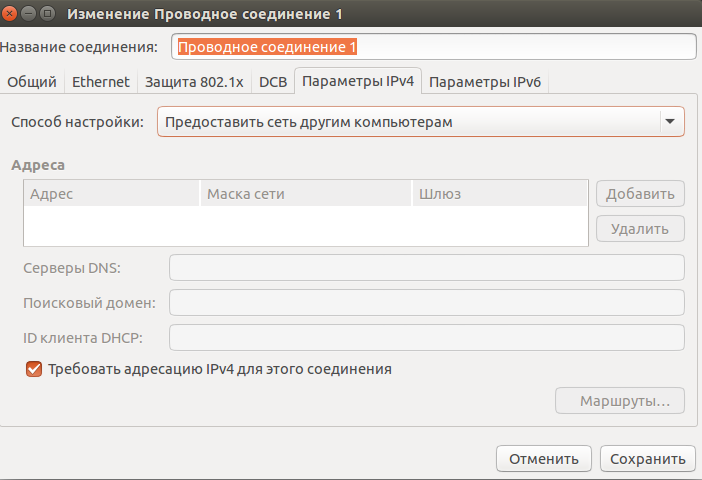
\includegraphics[width=0.6\linewidth]{network_1}}
\caption{ Параметры IPv4 для проводного соединения }
\label{network_1:network_1}
\end{figure}

\begin{figure}[h!]
\center{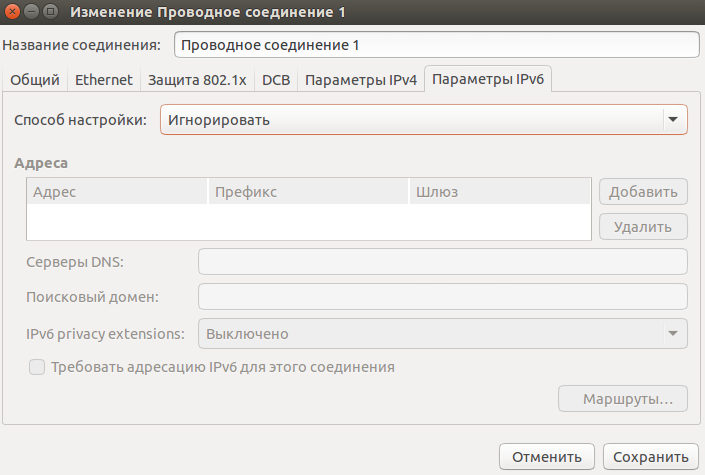
\includegraphics[width=0.6\linewidth]{network_2}}
\caption{ Параметры IPv6 для проводного соединения }
\label{network_2:network_2}
\end{figure}

\begin{figure}[h!]
\center{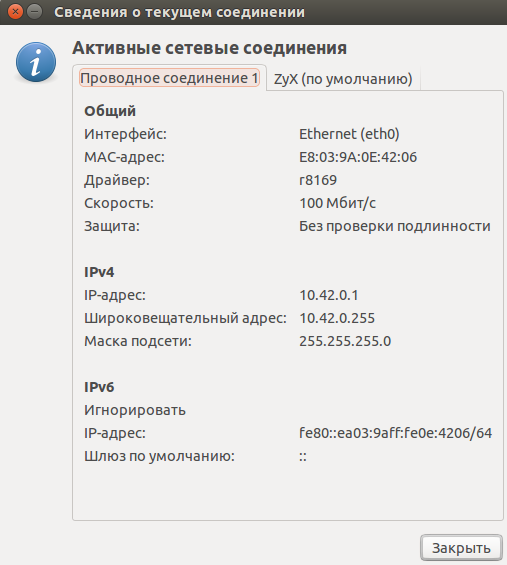
\includegraphics[width=0.6\linewidth]{network_3}}
\caption{ Сведения о проводном соединении }
\label{network_3:network_3}
\end{figure}

\clearpage




